\section{Motivation\label{sec:motivation}}
\begin{figure}[t!]
		\centering
			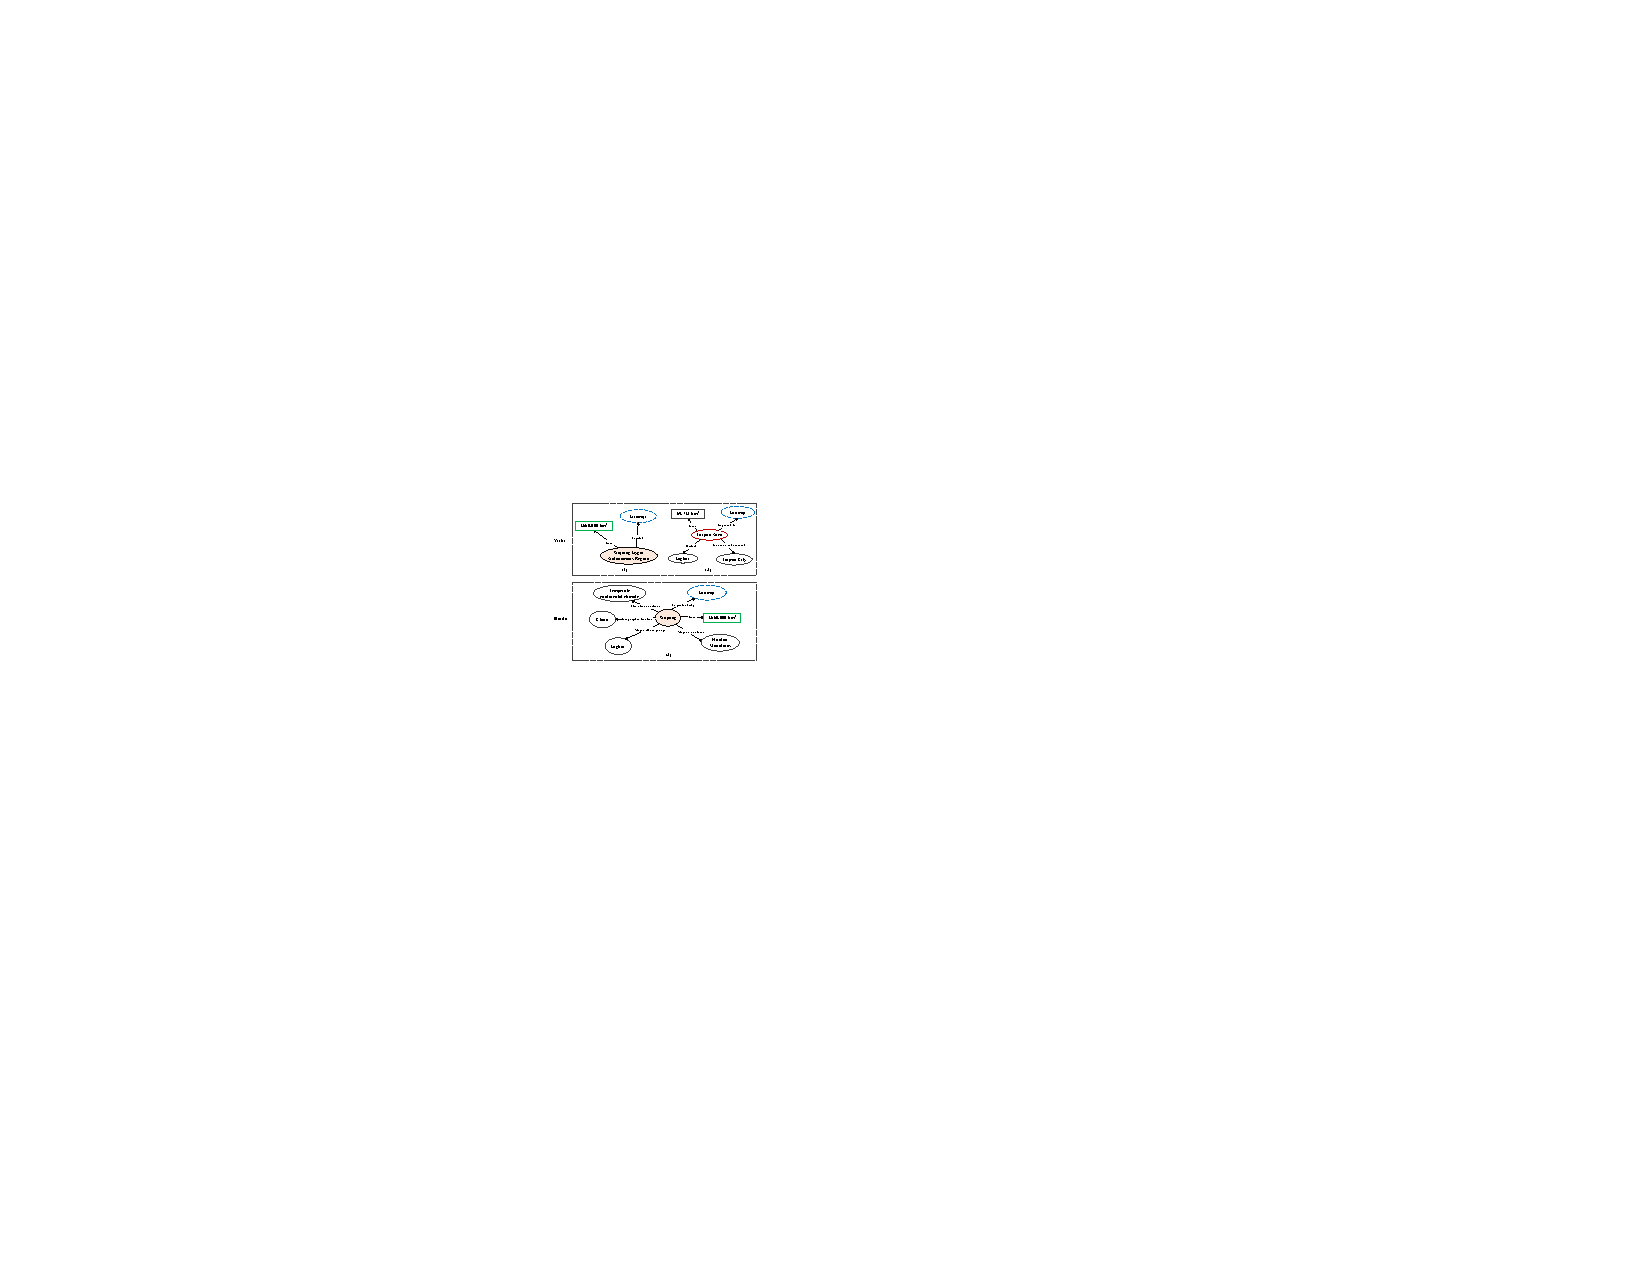
\includegraphics[width=1\linewidth]{figures/graph1.pdf}
			\caption{This example shows that the \emph{Xinjiang} entity from two heterogeneous \KGs (1 and 3) can be aligned using an entity (\emph{Urumqi}) and an attribute (1,660,000$km^2$), but existing methods all fail to align this entity.}
			\label{Xinjiang}
	\end{figure}
Consider Figure~\ref{Xinjiang} which depicts the heterogeneous neighborhoods of three center entities extracted from Wikipedia and Baidu
Baike (see Section~\ref{subsection:datasets}). In the diagram, an entity is marked by a circle and a value is indicated by a rectangle,
while a relation or attribute is listed on the edge.


The three neighborhoods have some entities (e.g., \emph{Urumqi}) and attributes (e.g., \emph{Area}) in common but their graph structure is
different. Specifically, \KGs (1) and (3) contain a common center entity of \emph{Xinjiang} (the surface form of this entity in Wiki is
\emph{Xinjiang Uygur Autonomous Region}). Therefore, a successful entity alignment strategy needs to link \emph{Xinjiang} from both \KGs.
However, state-of-the-art entity alignment methods~\cite{hao2016joint,chen2016multilingual,sun2017cross,zhu2017iterative} built upon TransE
all fail to align this entity because of two reasons: (i) they are misled by some of the redundant entities and attributes that only appear
in the Baidu dataset and (ii) they do not utilize attributes like \emph{1,660,000$km^2$}. This is a problem when using translation-based
embedding.

If we look closely into \KGs (1) and (3), we find that the \emph{Xinjiang} entity can be aligned using the entity \emph{Urumqi} together
with an attribute value \emph{1,660,000$km^2$}. In this example, if we give small weights to other entities and attributes, we can
successfully align the \emph{Xinjiang} entity.

This example shows that entity alignment requires one to carefully evaluate the importance of each entity and attribute from heterogeneous
\KGs. Unfortunately, this information varies across datasets and entities. Because manually obtaining this information for every target
entity would incur significant overhead, there is a critical need to automate the process. In this paper, we describe an novel approach to
offer this capability based on the \RGCN.
